%
% Chapter 1
%

\chapter{INTRODUCTION}
The recent observation of the Higgs boson confirmed the mechanism by which matter acquires mass. While this discovery made
significant progress towards completing the Standard Model's overall successful description of nature, many important questions
regarding the origins of mass remain unanswered. Do the observed properties of the Higgs boson match SM expectations? Why do
particles have the specific masses we observe? Is the top quark's large mass coming solely from its interaction with the Higgs?
Answering these questions will provide crucial insight into the underlying principles that govern our universe. The research and
analysis presented here attempts to address these questions. 

This analysis aims to discover processes from proton-proton collisions at the LHC where a Higgs boson is produced in association
with a top-antitop quark pair (denoted as \tth) and decays to final states with two or more charged leptons in the CMS detector
at a center-of-mass collision energy of 13 TeV.
Referred to as \tth multilepton processes, these provide an efficient probe with which to test the Standard Model. 

The purpose of \tth searches is to measure the top-Higgs Yuakawa coupling. While this coupling is already indirectly measured via tight constraints
on the gluon-gluon fusion production mode of the Higgs (where it is assumed a top quark dominates the loop), a direct measurement of this coupling
at tree-level is the ultimate motivation for \tth. 

There are significant experimental challenges to measuring \tth processes. Besides the large backgrounds and small signal, \tth events are themselves
complicated. There are 10 final state particles in the signal diagram in Figure~\ref{fig:intro_feyn}, this translates to at most 9 final state objects
reconstructed in the detector since the neutrinos are only detected due to a single missing transverse energy quantity. While having as many of the final
state objects as possible is desirable, it also makes the task of object assignment more complicated, since many objects are indistinguishable due to
finite detector resolution and uncertainties. This is also what makes reconstructing the visible Higgs mass nearly impossible. On the other hand,
events passing the signal region selection of this analysis rarely contain the full 9 objects due to a number of reasons. The missing objects could be mis-reconstructed
and not identified properly by the detector, or they fail the selection quality requirements, or they are outside the fiducial region of the detector
we restrict our search to. A full event reconstruction is also nearly impossible with missing objects also, and additionally the backgrounds look more similar
to partially reconstructed \tth signal events. 

\begin{figure}[hbtp]
 \begin{center}
   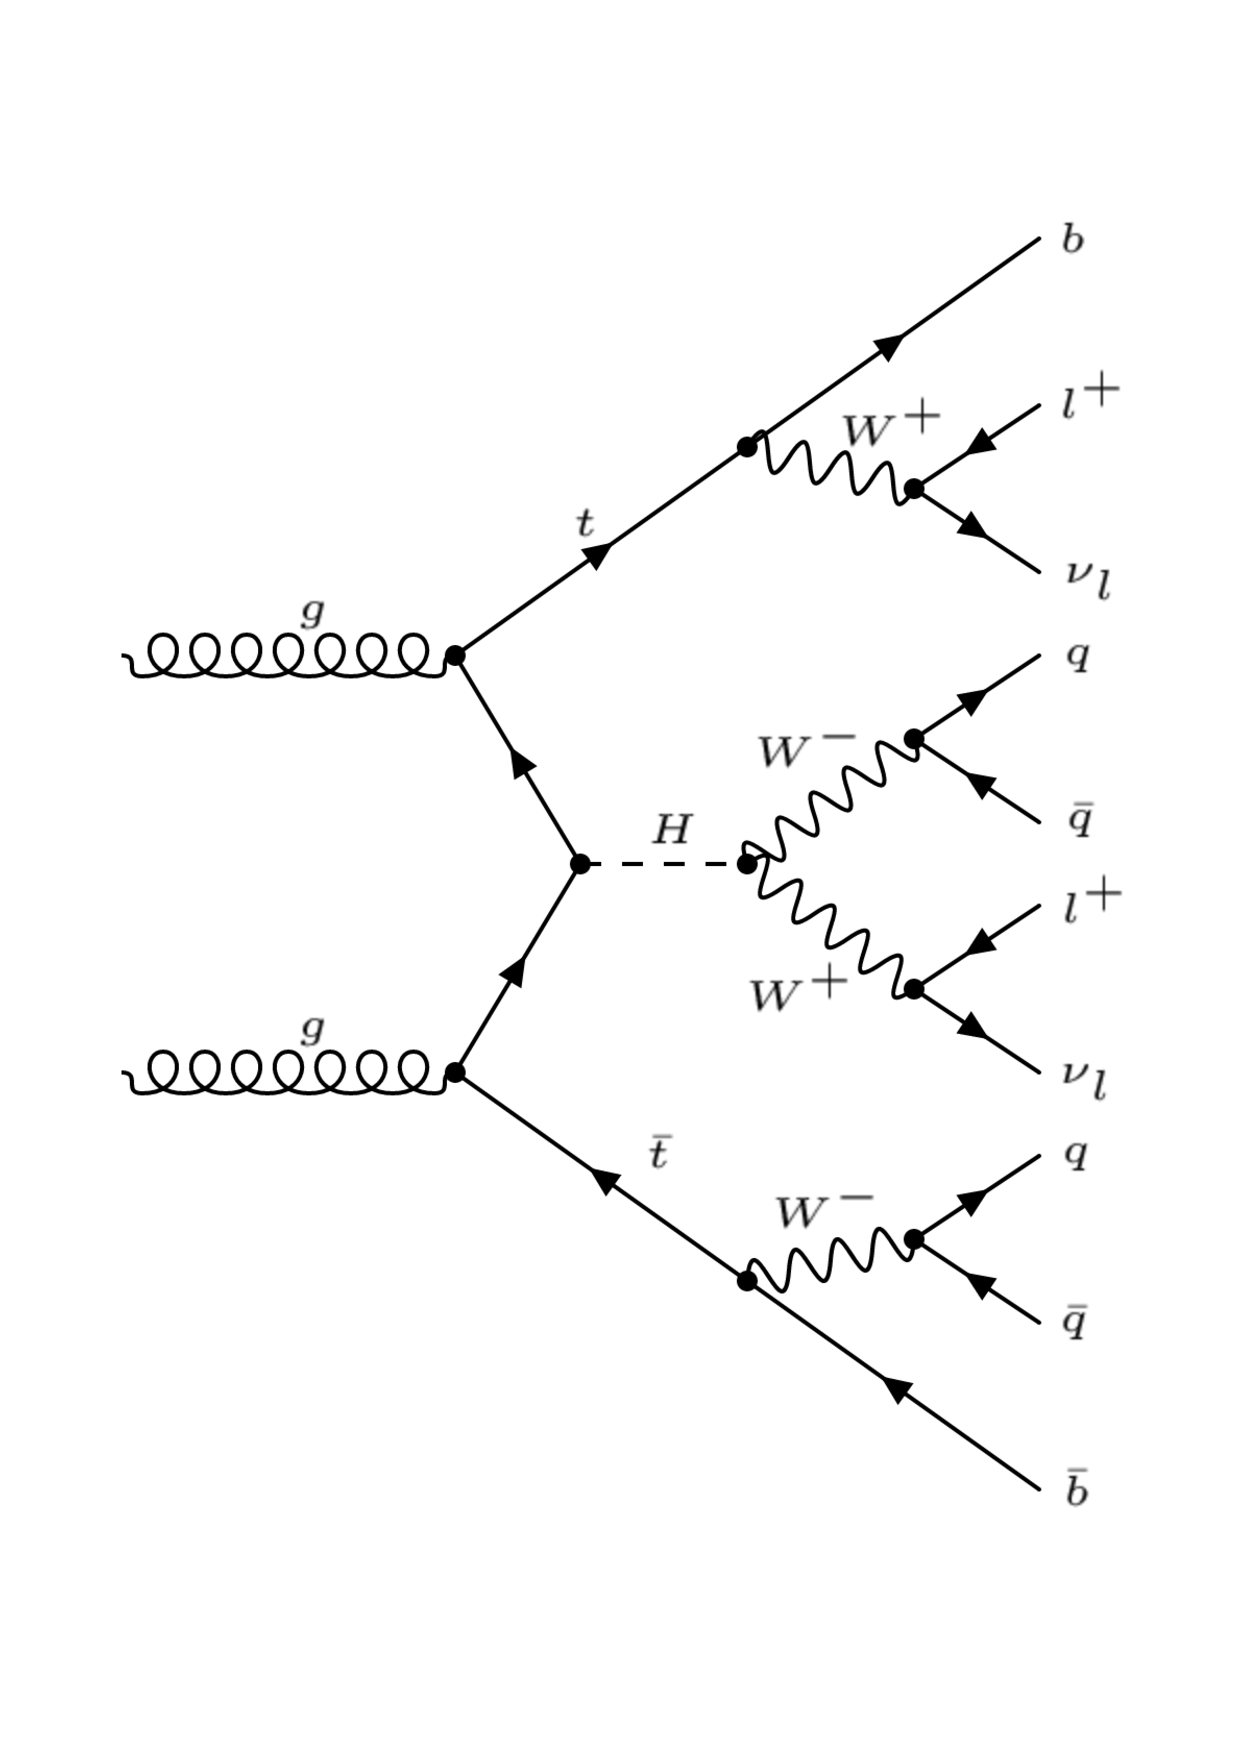
\includegraphics[width=0.5\textwidth]{ch1_figs/feynman_diagram_ttH_HWW_2lss.pdf}
   \caption[\tth feynman diagram]{A feynman diagram of the primary signal process.}
   \label{fig:intro_feyn}
 \end{center}
\end{figure}

There are several reasons for considering \tth events with multiple lepton final states. The primary experimentally-driven reason is due to the efficiency with which
CMS identifies and reconstructs charged leptons. Reconstructing electrons and muons accurately is far easier compared to reconstructing jets,
which will be discussed in the following chapters. 
From a theoretical perspective, the bb decay mode of the Higgs is the most desirable having the largest branching fraction, however this is balanced by the large
uncertainties and experimental difficulty of accurately identifying and reconstructing jets with CMS.
Finally, there tend to be smaller backgrounds capabable of producing multiple leptons consistent with \tth with respect to other Higgs decay modes. 

%%DISCUSSION OF PREVIOUS \tth RESULTS

The results presented here build on previous measurements of the top-Higgs Yukawa coupling that were performed in \tth analyses by both ATLAS and CMS.
The initial searches analyzed 20 fb$^{-1}$ of 8 TeV pp collisions during Run I of the LHC. Combining the results of Higgs decay channels of bb, $\gamma\gamma$,
and leptonic final states produced a signal strength of $\mu$ = 2.8 $\pm$ 1.0, where $\mu$ = $\sigma/\sigma_{SM}$. The multilepton channel alone
observed $\mu$ = 3.7$^{1.6}_{1.4}$~\cite{jhep_tth}. Subsequent iterations of the multilepton analysis were performed again on 13 TeV pp collisions from Run II
of the LHC, the most recent signal strength observations are $\mu$ = 2.0$^{0.8}_{0.7}$, corresponding to 12.9 fb$^{-1}$, and the subsequent analysis on the full
2016 dataset on which this dissertation is based, and $\mu$ = 1.5 $\pm$ 0.5 ,corresponding to 35.9 fb$^{-1}$.


% % uncomment the following lines,
% if using chapter-wise bibliography
%
% \bibliographystyle{ndnatbib}
% \bibliography{example}
